In this section, the reader will be introduced to the proceedings in science which are
relevant or related to this thesis. They are grouped into the following topics of interest:

\begin{itemize}
	\item \textbf {Motivation for the topic of this thesis} - Provides an explanation on why the chosen topic of this thesis is generally of interest, and why similarity measures in music are feasible (given optimal circumstances).
	\item \textbf {Features of digital music} - Gives an overview of existing methods of feature extraction which are purely based on computational methods.
	\item \textbf {Subjective music similarity computation} - Lists literature which is related to this thesis' problem of computing the subjective similarity of artists, which is based on subjectiveness as experienced by humans.
	\item \textbf {Visualization of artist similarity} - Provides an overview of existing methods and models of visualization of music similarity (or, in this case, artist similarity).
\end{itemize}

\section{Motivation for the Topic of This Thesis}

Music is an integral part of the daily life in nearly all societies, and the list of published titles is growing every day. As huge amounts of data tend to be hard to digest, a promising approach is to create ontologies by which music can be categorized in a hierarchical fashion. Aside from the general motivations for this thesis presented in Chapter ~\ref{ch:intro}, the motivation to choose music similarity as a means of ordering music has its roots in recent resesarch. The categorization of arbitrary music titles is neither implicit nor trivial, and music similarity has been a promising metric which can be derived from usage data, as opposed to deriving it from analysis of music bitstreams. Serving the demands of Electronic Music Distribution (EMD), the authors of \cite{pachet:02g} elaborate on the feasibility of music similarity measures. It is found in \cite{pachet:02g} that the introduced similarity measure (timbre similarity) combined with other measures can yield interesting results. It is also mentioned that the interpretation of experimental results in the field of music similarity is challenging due to the subjective demands. 

It is clear that even the best-educated music experts could hardly agree on 
any distinct similarity measure between two music titles, due to the implicit fuzziness of subjective measures. In \cite{Ellis02thequest}, it is mentioned that a simple mistake as overlooking an artist when rating similarities can severely change the results. For this reason, it can be assumed that it is rare that two humans would agree on the same similarity between music files
if they voted independent of each other.

As mobile devices are becoming increasingly ubiquitious, this thesis is focusing on strategies and implementations of music similarity for mobile computing.

\section{Features of Digital Music}

As opposed to subjective artist similarity, there are music features or measures which can be retrieved by purely computational approaches. In the field of audio feature extraction, a wide range of feature extractors has been created. Feature extractors perform bitstream analysis of digitally stored music files and extract one or more reproducible measures characterizing the file. Subsequently, the music files can be classified by the features. Interestingly, it is confirmed in \cite{LID_05ismir} that the use of psycho-acoustic enhancements before feature extraction improves the classification accuracy significantly. It can be concluded that the outcomes of audio feature extraction are influenced by many factors which are not always intuitive.
As has been mentioned previously, most audio classifiers analyze the bitstream of music files - however,the bitstream is only one dimension of a piece of music, if we regard it as a multidimensional object. For example, it is also possible to analyze the lyrics, as has been done in \cite{DBLP:conf/ismir/MayerNR08}. Feature extraction typically requires a lot of computational effort before similarity between two audio streams can be determined (which still is not guaranteed to represent human subjective similarity). However, the time it takes an app until the user can interact with it is an important feature in usability. Therefore, other approaches to similarity retrieveal which have lower computational impact should be preferred to feature extraction.

\section{Subjective Music Similarity Retrieval}

Subjective similarity, as the author understands it, expresses human opinions on a certain object. As previously mentioned, it is obvious that humans will hardly agree on attributes of music, and the same person might even make different statements in the course of time, depending e.g. on her mood. The following applies to both artist 
similarities and music file similarities, since the former may be constructed from aggregations of the latter (it has to be noted at this point that many artists tend to produce music from multiple genres, thus making an artist-to-artist-comparison difficult or even infeasible). In article \cite{Ellis02thequest} it is found that it is doubtable that a common ground truth for subjective artist similarity even exists, because of the inhomogeneity of measures made by the involved users. It can be deduced that a meaningful model of subjective music similarity will in most cases only resemble a compromise between different stakeholders.
As inferred from \cite{Berenzweig03alarge-scale} and \cite{mcfee09_hesas} there are different approaches to retrieving a model of subjective similarity for a given set of music files, which include:

\begin{itemize}
	\item Conduction of surveys with end users
	\item Opinions of experts
	\item Co-occurrence of songs and/or artists in end users' libraries or playlists
	\item Data mining of text in web sources (e.g. lyrics, artist biographies, etc.), as performed in \cite{Whitman02inferringdescriptions}
	\item Leveraging data gathered by social music services
\end{itemize}

As it is intended by this thesis to provide a concept for a fast and fully automatic approach to similarity measuring, we will concentrate on the last approach, the usage of data provided by social music services. Hybrid computation methods, such as the method described by \cite{mcfee09_hesas} (combining acoustic features with text excerpts and tags retrieved from online services) turn out to be hardly feasible on a mobile device because of performance requirements. It is assumed by the author that for a rough estimation of music file or artist similarity, the data provided by social music services (as opposed to hybrid approaches) is sufficiently meaningful, as their daily user base is in the millions and still growing.

Apart from the source of similarity metrics, also the scope of computation has to be given thought to. Depending on a user's scenario, the user might want to explore her own music collection, or she might want to discover music similar to her own. In the following subsections, both cases are considered.

\subsection{2D-Projection of Collections of Music}
\label{subsec:2dprojection}

In order to provide a meaningful, semantic overview of a collection of objects, data must be available or generated for all objects in the collection, or for most of them. 
As has been mentioned before, \textbf{extraction of features} of music files may be used to gather metrics about the analyzed files. The data retrieved can then be combined into a feature vector of N dimensions, where N is the number of features. When all files in the analyzed music collection have been classified in this way, a \textbf{self-organizing map} or other mapping algorithms is then applied and trained with the resulting feature vectors, mapping vectors with small Euclidean distances spatially near to each other \cite{RAU_02ismir}. This results in a map where elevation represents the frequency of vectors in certain areas - thus, a high elevation at a point on the map means that the feature vector attached to the point is similar to a big number of music files. It is obvious that self-organizing maps are well suited for visually clustering music files by their features. However, it must be noted that this approach is only feasible if a huge amount of music metadata 
can be retrieved, either by feature extraction (which has been put aside for this thesis because of computational time reasons) or other methods like text mining. Because of these dependencies, self-organizing maps are not optimal for this thesis. 

Another broad group of similarity/dissimilarity visualizations is made up of \textbf{force-directed graph layouts}. They all consist of nodes, which are representations of music objects, and edges, which map to relations between music objects. Consequently, a graph is a visual representation of a collection of music objects. The distances (edge lengths) between nodes approximate a function over the previously determined dissimilarities between the music objects. As has been described in \cite{gansner:1998}, the application of pseudo-physical forces on an undirected graph provides for a improvement of the graph layout. This is achieved by adding attractive or repulsive forces to all nodes in the graph, such that nodes push away from or attract each other. As long as there is energy left in a graph (i.e., there are objects which are not in their optimal position), the nodes are moved in a way that satisfies the applied forces. The authors of \cite{Muelder:2010fk} have described and experimented with several graph-based layouts, and among them was a force-directed layout algorithm called LinLog \cite{noack:2003}, which has been found to deliver the most esthetic results. However, a computational model which is more suitable for the calculation on mobile devices is presented in \cite{Kobourov04} on page 4. This concrete algorithm for \textbf{continuous calculation of a force-directed graph layout} will be used for the display of loose, unranked objects in this thesis, especially in the context of artist discovery (more about this later in this section).

Force-directed algorithms, as described in the previous paragraph, do not necessarily reflect semantic meaning in their resulting layouts. However, for cases where semantic meaning must be conveyed - as in the display of artist similarity - other approaches to force-direction exist. A special form of multi-dimensional scaling (MDS) is based on \textbf{spring models}, which also produce layouts by applying forces.
Multidimensional scaling means the translation of objects in a high-dimensional space into another space of more or less dimensions. Most often, MDS is used to map objects from a very high dimensional space into a two- or three-dimensional space, in order to make their relative positions to each other comprehensible to humans. Dimensions in this context do not have to be spatial, or even continuous - a dimension in this sense can be any attribute which all objects in the observed set have in common (or which can be assigned to all objects). In order to eliminate or aggregate dimensions (as must be done to reduce dimensionality), several techniques have been found.
As mentioned above, the most promising for the objective of this thesis, is the adoption of a spring model.

Multi-dimensional scaling supported by spring models depends on a \textbf{similarity matrix} containing all objects of the analyzed music collection. A similarity matrix contains the similarities (or rather the dissimilarities) of all items to each other, in the form of distances. Intuitively, the measured item-item distance is higher if they are more dissimilar to each other (a distance of zero expressing equality between items). Data sources for similarity matrices describing music include 
(as described earlier in this chapter):
\begin{itemize}
	\item Surveys, playlist co-occurrences, user collection co-occurrences, web text mining,... 
	\item Similarity rankings or measures from public Web APIs
\end{itemize}
As mentioned before, we will concentrate on the latter (similarity measures from public Web APIs) for complexity reasons. The task of building up a similarity matrix for a collection of music titles is then reduced to a number of Web API calls, mapping the resulting distances or rankings to the objects in the collection. The similarity matrix is then used in order to find a suitable two-dimensional representation in Euclidean space, where the spatial distance between objects represents their similarity, or their dissimilarity respectively.

The process of finding a suitable two-dimensional representation with a spring model will now be described. The spring model algorithm emulates the physical behavior of steel rings connected by metal springs (as shown in Figure ~\ref{fig:spring_model}). To continue with the analogy, the algorithm starts off with the steel rings at random positions, and in multiple iterations tries to satisfy the springs' forces. A spring's force is usually proportional to the discrepancy of two objects' high-dimensional distance and their low-dimensional distance. The fitness of the model (all steel rings being at their optimal position, considering all connected springs) is described by a stress function. The lower the stress function's output, the better the new low-dimensional model suits the original high-dimensional model. In most cases a perfect match between high-dimensional and low-dimensional Euclidean distances (stress function output = 0) is not possible, and thus for the algorithm to terminate, sensible termination criteria have to be defined - e.g., if the velocity of objects moving at each iteration falls below a predefined threshold, the algorithm terminates and the resulting low-dimensional representation is accepted as being "'good enough"'.

\begin{figure}[H]
  \centering
    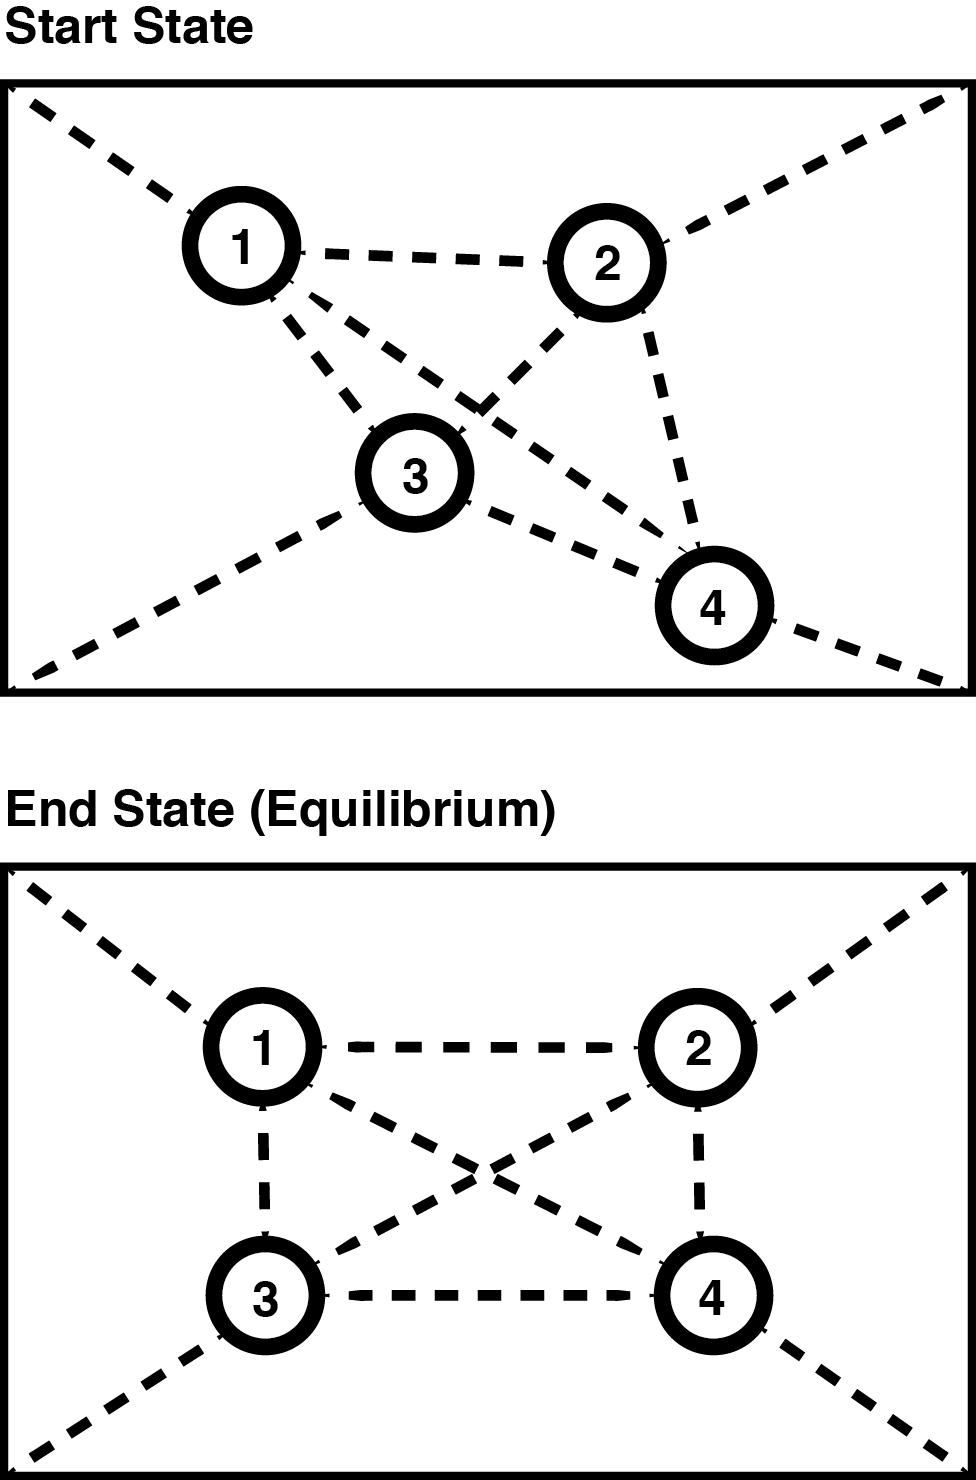
\includegraphics[width=0.45\textwidth]{figures/spring_model}
  \caption{Steel Rings Interconnected By Springs Which Pull At Each Other Until They Reach an Equilibrium.}
  \label{fig:spring_model}
\end{figure}

Unfortunately, naïve versions of spring model algorithms are inflexible in the sense that the whole algorithm has to be executed all over again if slight changes to the data set occur \cite{Morrison:2003:FMS}. Therefore, a computationally advantageous and more flexible approach to spring model algorithms has been presented in \cite{Morrison:2003:FMS}, combining it with \textbf{sampling and interpolation}. As opposed to naïve spring model algorithms, this hybrid methodology starts off with a random sample of size $\sqrt{N}$, where N is the number of objects contained in the dataset. After the naïve spring model computation (the version described in the last paragraph) has been performed on only the subset, the rest of the data set ($N - \sqrt{N}$ objects) is integrated into the low-dimensional model by an interpolation process which is described in detail in \cite{Morrison:2003:FMS}. It has been found in the article that this combination of algorithms improves greatly on the accuracy of the model (i.e., a lower stress function output) and offers a sub-quadratic run time of $\mathcal O(N*\sqrt{N})$, as opposed to a run time of $\mathcal O(N^3)$ or $\mathcal O(N^4)$ with a naïve spring model alorithm.

\subsection{Discovering Objects Similar to a Given Object}

After the elaboration of means of exploring the semi-static collection of objects in a user's library, heed must be given to the recommendation of unknown objects. Equipped with similarity data retrieved from various web APIs it is not only possible to compute relations of objects within a library, but also to find related objects which are currently not present in the library. It is clear that the same algorithms which have been previously described would compute usable outcomes by simply adding unknown objects to a library's representation (e.g. spring model MDS); yet, it can be assumed that in most cases only one object in a library is the starting point of a search for similar objects. This renders a big part of the library's representation irrelevant for this use case - consider a user searching for interprets similar to "'The Beatles"' - most likely, she will not be interested in how these unknown interprets relate to other bands in her library. Also, integrating such previously unknown objects into the representation of a big library will be computationally and query-wise too complex in this scope, as dissimilarity distances to all objects in the library have to be determined. It must be noted that the representation for unknown object recommendation can only be a rough approximation (because of the previously described volatility of subjective similarity), and for this reason not only numerical measures, but also similarity rankings are considered sufficient for this use case.

A computationally less expensive algorithm for such means has been proposed in \cite{Marshall:2010}, consisting of a fusion of similarity rankings from various social music services. In this article it is demonstrated that various methods of embedding (fusing) similarity rankings from online services can provide different meaningful similarity models, some of which give more weight to unknown artists. This methodology is able to compute a ranked list of similar objects, based on multiple sources for greater reliability, in a customizable way. The fusion methods reach from rank-average to concordet-fusion (unweighted directed graph). Three major benefits speak in this approach's favor over global numerical similarity measurements:

\begin{itemize}
	\item \textbf{Potentially insignificant computation times} while preserving a stable similarity ranking very well suited for mobile end users.
	\item \textbf{Simple but effective customization} achieved by easily exchangeable fusion algorithm components.
	\item \textbf{Reducing the number of web API queries to a minimum} greatly reduces the overall number of network requests, making the method faster and even better suited for mobile usage.
\end{itemize}

It must be noted though that the rank fusion algorithm is neither able to define distances between arbitrary objects in the dataset - only a dissimilarity ranking between the starting point object (e.g. "'The Beatles"') and the remaining objects is obtained - nor is it able to force the inclusion of objects (from a local library) in the ranking. Therefore, it is only kept here as a related reference, but cannot be applied to this thesis. Instead, in cases where it is necessary, similarity values from various web sources will be combined by calculating their mean - for example, if Last.fm reports that "'The Beatles"' and "'The Who"' share a similarity of 0.8, and Echonest claims a value of 0.7 for that same artists, then the resulting value will be 0.75.

\section{Visualization of Artist Similarity}

The mode or fashion of data visualization can be considered a crucial aspect of interfaces for humans (i.e., graphical user interfaces). Today, humans' ability to apprehend information presented to them is limited in several ways, some of which are physical, and some of which are of psychological nature. Some of these limiting factors include:

\begin{itemize}
	\item Restriction of short-term memory,
	\item Limited power of concentration,
	\item Narrow attention span (especially while using mobile device),
	\item Color blindness,...
\end{itemize}

Therefore, it is desirable to give heed to the choice of visualization method to achieve optimal apprehension results, without hindering information understanding through visualization errors. Since the field of music and music collection visualization is broad and not all algorithms can be presented within this thesis, the author decided to select only the field of two-dimensional collection visualizations for further investigation. It must be noted that several fields of visualizations are left out of the scope here, including:

\begin{itemize}
	\item \textbf{Abstract visualization as an art form} - Certain art forms try to make music more tangible by creating matching images, as in the movie "'2001 - A Space Odyssey"' by Stanley Kubrick, or in works by the demo scene in Germany \cite{Scheib:2002}.
	\item \textbf{Realtime computed images as abstract visualization} have become common components of many desktop audio players, presenting the user with animated images (fractals, 3D-animations,...) which somehow resemble certain features of the currently played music.
	\item \textbf{3D environments resembling music content} give users the ability to roam through a virtual space similar to the way they interact with the physical world, as described in \cite{Dittenbach:2007}.
\end{itemize}

The scope of this thesis confines itself to the visualization of music tracks as objects, relating these objects to each other, and disregarding their real-time aspects (i.e., not generating any visualizations during playback). Intuitively, the computation and visualization of those relations (also, the quality of relations, e.g. ranking or dissimilarity distances) are closely related to each other. In some cases, a certain mode of computation of object relations more or less forces or forbids the usage of certain visualization approaches. Therefore, the presented modes of visualization are at least closely related to their computational counterparts from the previous subsection.

\subsection{Visualization of Collections of Music}

Previous work has shown that \textbf{self-organizing maps (SOM)}, which are in this context also called "'islands of music"' are well suited as visualizations of related music objects \cite{Cooper:2006:VAM}. This methodology depends on raw audio stream analysis (performed by aforementioned feature extraction algorithms), and subsequently displaying them on an elevation-map, similar to a geographical map. Proof-of-concepts have been successfully implemented, as has been demonstrated in \cite{NeuDitRau_05ismir}, featuring the PlaySOM. The information such self-organizing map visualizations want to give the user is: There are clusters of similar pieces of music in the provided collection, and within one cluster the contained music files most similar to each other. Additionally, each cluster has its own weight vector which can be used to add semantic height annotation to the map - clusters where similar values of a certain feature are especially concentrated receive a "'high"' or "'hot"' profile, whereas value ranges of that feature which are uncommon receive a "'low"' or "'cold"' profile.

Other graph layouts which pose options for music collection browsing include \cite{Muelder:2010fk}:

\begin{itemize}
	\item Principal Component Analysis (PCA) layouts 
	\item Tree map layouts 
	\item Space filling curve layouts
\end{itemize}

However, the most promising visualization in this context, namely \textbf{2D layouts generated via multi-dimensional scaling}, has already been discussed in ~\ref{subsec:2dprojection}. They can be created without putting too much strain on mobile device processors.

\subsection{Visualizations for the Recommendation of Unknown Objects}

As has been discussed in the previous subsection, the computational approaches for the recommendation of new objects can be either very similar to the computation of ordinary collection visualization, or they can use more simplified rank-based models. The former are clearly covered properly by the broad range of previously described visualization methods for collections of objects. On the contrary, visualization possibilities for rank-based computation models are not as manifold, due to the fuzzy dissimilarities between objects - a ranking can not be used to acquire deterministic object distances. However, since the goal of the visualization of such a ranking is to provide a very rough overview to the user, a deterministic visualization is not necessary. Therefore, for this thesis, ranking of related artists is omitted, and related artists are displayed as relations with equal importance, as has been done by the authors of \cite{DBLP:conf/webist/SarmentoGCO09}. For this use case, a force-directed graph layout provides for the most esthetic results \cite{DBLP:journals/spe/FruchtermanR91}. Additionally, such layouts can execute their self-optimization in realtime while being presented to their user without affecting the user experience in a negative way, as is shown by \cite{url:tuneglue}. Further on, the nodes in such layouts are user-manipulable in realtime. For these reasons, it is valid to omit rankings of related artists when displaying them, but further research should concentrate on how rankings can be integrated into artist discovery without harming the user experience.

\section{Summary}

The reader has been introduced to related work in the domain of this thesis. Music is an integral part of our society, and while measuring similarity between pieces of music is possible, categorization of titles is challenging due to music's subjective nature. It has been asserted that the bitstream of a title is only one dimension from which features can be extracted - e.g., lyrics sourced from the Web can also be used for feature extraction. For the use of similarity as a semantic enhancement of music collections, computation of layouts based on subjective similarity metrics has been explored extensively. Based on the assumption that deterministic similarity data is present, computational methods have been described - self-organizing maps and multi-dimensional scaling. Multi-dimensional scaling, being the most fitting method for the context of this thesis, will be used later on.

In the context of music discovery - finding objects related to a distinct music object - an algorithm has been referenced which fuses similarity rankings between music objects, potentially enabling display of ranked similarities. However, for the context of this thesis, ranked similarities are omitted, and artists will be shown unordered. Using ranked similarities while discovering artists should be part for further research.

For the visualization of previously mentioned music collections (enhanced with similarity data), methods like self-organizing maps, force-directed graph layouts, and spring models (based on multi-dimensional scaling) have been referenced. As mentioned before, multi-dimensional scaling and the resulting visual representation will be used here.